%!TEX root = thesis.tex
\chapter{Cryptographic Primitives}
\al{check usage of i.e. and e.g.. Pretty sure I abused them at some points}
Secure function evaluation (SFE) is the study of computing functions in a secure fashion. 
SFE can be split into two cases: cases where there are two parties involved, referred to as two-party computation (2PC), and cases where there are three or more parties, referred to as multiparty computation (MPC).
This thesis will focus primarily on 2PC protocols, but many of the methods are applicable to MPC as well.

2PC protocols are complex cryptographic protocols that rely on a number of cryptographic primitives.
In order to understand 2PC, it is not crucial to understand how the cryptographic primitives work, but it is important to understand their inputs, outputs and security guarantees. 
This first chapter will give an overview of the cryptographic primitives used in 2PC protocols.

\section{Computational Indistinguishability} 
\label{sctn:computational-indistinguishability}
Computational Indistinguishability is a method of mathematically justifying the hardness of an algorithm to break. 
At a high level, we say that two sets are indistinguishable, if there is no efficient algorithm that can tell the two sets apart. 
We present the definition formally here, but it is best understood when it is used to define and prove the security of particular schemes. 
In section \al{add label/ref} we use computationally indistinguishability to show that an encryption scheme is secure, and in section \al{add label/ref} we use it to show a 2PC protocol is secure. 
\al{does the term ''break`` seem meaningful here? At some point, at least, I should be clear about what it means.}

We formally define computational indistinguishability as follows.

 \al{should this be a definition section?}
 
 \begin{definition}
 \label{defn:computational-indistinguishability}
Let $\mathcal{X} = \{X(n,a)\}_{n \in \NN, a \in \{0,1\}^*}$ and $\mathcal{Y} = \{Y(n,a)\}_{n \in \NN, a \in \{0,1\}^*}$ be distribution ensembles.
$\mathcal{X}$ and $\mathcal{Y}$ are computationally indistinguishable, denoted $\mathcal{X} \compindist \mathcal{Y}$, if and only if for all non-uniform polynomial-time distinguisher $D$, there exists a function $\mu(\cdot)$ that is negligible in $n$, such that for all $a \in \{0,1\}^*$, 
\begin{equation}
    |Pr[D(X(n,a)) = 1] - Pr[D(Y(n,a)) = 1]| < \mu(n)
\end{equation}
\cite{lindell2009secure}.
\end{definition}

\begin{definition}
\label{defn:negible}
A function $\mu : \NN \to \RR$ is negligible if for all positive polynomial $p(\cdot)$, there exists positive integer $N_p$ such that for all $x > N_p$, 
\begin{equation}
    |\mu(x)| < \frac{1}{p(x)}.
\end{equation}
\cite{goldreich}
\end{definition}

\section{Encryption}
Encryption is the process of encoding a message such that only parties with the key can read the message.
As we discuss 2PC, we will be using symmetric-key encryption, the case where encryption and decryption use the same key.
A symmetric-key encryption protocol is composed of two parts.
The first part is the encryption algorithm which obfuscates the message, and the second part is the decryption algorithm which unobfuscates the disguised message.
The encryption algorithm is denoted $\Enc$, and the decryprtion algorithm is denoted as either $\Dec$ or $\EncInv$.
\begin{equation}
    \label{eqn:encryption}
    \begin{split}
        \Enc_k (pt) & = ct  \\
        \Dec_k(pt) = \EncInv_k(ct) & = pt
    \end{split}
\end{equation}
where $pt$ is the original message or the \emph{plaintext}, $ct$ is the encrypted message or the \emph{ciphertext}, and $k$ is the secret key.
For the algorithm to be effective, the secret key $k$ must be randomly sampled from $\{0,1\}^\lambda$, where $\lambda$ is the security parameter of our protocol.\footnote{The notion of randomness in cryptography is precisely defined, and in cases where $\lambda$ is large, it is sufficient for $k$ to be pseudorandom. Pseudorandomness is also precisely defined.}
\al{does footnote go before or after period? ShouldI have footnotes?}
If  $\lambda$ is increased, thereby increasing the size of the key, then the encryption algorithm becomes harder to break.
We will not go into details about how encryption algorithms are instantiated; we will merely treat them as algorithms which we can use at our leisure.

We say that an encryption scheme is secure \footnote{Specifically, this is the definition of a chosen-plaintext-attack secure encryption scheme. There exists weaker and stronger definitions of security, but chosen-plaintext-attack security is frequently used for 2PC}, if the following game is true:

% TODO WORK HERE
\al{Get crypto book and finish this}

\begin{definition}
Define the following game:
What are the inputs?
\begin{enumerate}
\item Adversary picks two messages $m_0$ and $m_1$, and gives $m_0$ and $m_1$ to the sender. 
\item The sender samples $k \gets \{0,1\}^{\lambda}$ and $b \gets \{0,1\}$. The sender gives $m_b$ to the adversary. 
\item The adversary may spend a polynomial amount of time doing computation. Eventually, the output $b'$, their guess as to which message they received.
\end{enumerate}
\end{definition}
% END WORK HERE

It is useful for 2PC to define a specific type of symmetric-key encryption algorithm called a Dual-Key Cipher (DKC) \cite{bellare2012foundations}.
A DKC requires two secret keys to encrypt and decrypt the message, in contrast to classic encryption which only requires one.
It is easy to instantiate a DKC if one has a secure encryption scheme: let $k_0$ and $k_1$ be the two secret keys and instantiate the DKC as follows:
\begin{equation}
    \begin{split}
        \EncDKC_{k_0, k_1}(pt) = \Enc_{k_1} ( \Enc_{k_0} ( pt )) \\
        \EncDKCInv_{k_0, k_1}(ct) = \EncInv_{k_0} ( \EncInv_{k_1} ( ct )) 
    \end{split}
\end{equation}
This construction of a DKC is slow, and there are many faster methods for instantiating DKCS.
For more information, see \cite{bellare2012foundations}.

\section{Boolean Circuit} 
A function in a 2PC protocol is represented as a boolean circuit.
A boolean circuit takes as input $x \in \{0,1\}^n$, performs a series of small operations on the inputs, and outputs $y \in \{0,1\}^m$.  
You may have encountered circuits and logical operators in another context, where the inputs and outputs were True and False.
For our usage, True will correspond to the value $1$, and False will corresond to the value $0$. 

The small operations done inside of a circuit are performed by a \emph{gate}.
A gate is composed of three wires: two input wires and one output wire, where a \emph{wire} can have a value either $0$ or $1$.
A gate performs a simpler operation on the two inputs, resulting in a single output bit.
Table \ref{tab:xor} gives the mapping of an XOR gate.

\begin{table}[h]
\label{tab:xor}
\centering
\begin{tabular}{ | l | c || r |}
\hline
x & y & xor(x,y) \\ \hline
1 & 1 & 0 \\ \hline
1 & 0 & 1 \\ \hline
0 & 1 & 1 \\ \hline
0 & 0 & 0 \\ \hline
\end{tabular}
\caption{The mapping of an XOR gate.}
\end{table}

A circuit is a combination of gates that are stringed together.
It turns out that circuits are quite powerful: in fact, a circuit composed only of AND gates, XOR gates and NOT gates can compute any function or algorithm \cite{Goldreich}.
In other words, if there's some algorithm that can do it, then there is some circuit that can do it as well.
Figure \ref{fig:less_than_circuit} shows the circuit representation of the less than function, $f$ as specified in equation \ref{eqn:less_than}.

\begin{figure}[h]
    \centering
    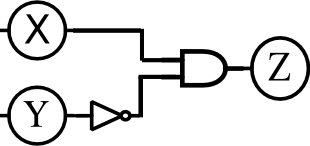
\includegraphics[scale=0.75]{images/drawing.png}
    \label{fig:less_than_circuit}
    \caption{A circuit that computes the less or equal to function, equivalent to the less than function for input of two one-bit values.}
\end{figure}

\begin{table}[h]
\label{tab:less_than}
\centering
\begin{tabular}{ | l | c || r |}
\hline
x & y & $x < y$ \\ \hline
0 & 0 & 0 \\ \hline
0 & 1 & 1 \\ \hline
1 & 0 & 0 \\ \hline
1 & 1 & 0 \\ \hline
\end{tabular}
\caption{The truth table of the less than circuit.}
\end{table}

\section{Oblivious Transfer}
\al{more sources here - get from CompGC paper}
Oblivious Transfer (OT) is a two-party protocol where one party (sender) has two inputs, $m_0$ and $m_1$, and the other party (receiver) has a bit $b \in \{0,1\}$. 
OT enables the receiver to acquire $m_b$ from the sender without revealing which message is received, i.e., the value of $b$.
Moreover, the receiver learns nothing about the message that isn't received, i.e. anything about $m_{1-b}$.

Here we give the Naor-Pinkas protocol of $1-2$ oblivious transfer.
The protocol relies on the DDH assumption.\footnote{The Decisional Diffie-Hellman (DDH) assumption is a computational hardness assumption involving discrete logarithms in cyclic groups. For more information, see \cite{Boneh1998}.}

\al{Should I give the full protocol? Probably shouldn't have a screenshot of wikipedia in the thesis}

\begin{figure}
    \centering
    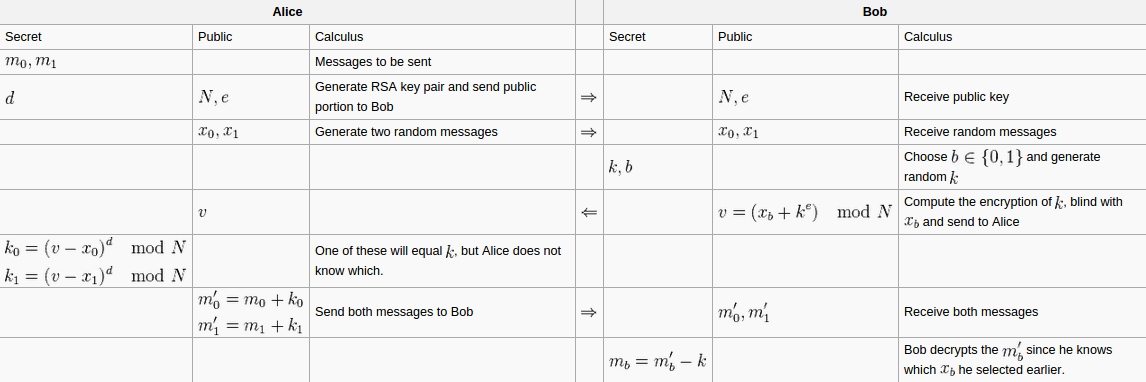
\includegraphics[scale=0.3]{images/ot_wiki}
    \caption{Semi-honest Naor-Pinkas oblivious transfer.}
\end{figure}

Oblivious transfer has been improved in two relevant ways for 2PC protocols. 
These improvements are called OT-extension and OT-preprocessing. 
In OT-extension a constant number of OT's can be run to generate a polynomial number of exchanged values.
In OT-preprocessing the OT's occur before the actual protocol, during what is called the offline phase, and then when the OT's needed during the online phase, simpler and efficient communication realizes the exchanged values.
This is useful because the OT step requires a large amount of communication to be sent between the sender and receiver, often resulting in OT being the bottleneck of 2PC protocols.
